\documentclass{article}
\usepackage[table]{xcolor}
\usepackage{array}
\usepackage{float}
\usepackage{graphicx}
\usepackage{tikz}
\usepackage{tcolorbox}
\usepackage{amsmath}
\usepackage{enumitem}
\usetikzlibrary{trees, arrows.meta}
\usepackage{listings}
\usepackage{xcolor}
\usepackage[utf8]{inputenc}   % Suporte para codificação UTF-8
% Definir um verde mais suave
\definecolor{mygreen}{rgb}{0.1, 0.6, 0.1}
\lstset{
    language=Python,
    basicstyle=\ttfamily\footnotesize,
    keywordstyle=\color{blue},
    commentstyle=\color{mygreen},
    stringstyle=\color{red},
    numbers=left,
    numberstyle=\tiny\color{gray},
    stepnumber=1,
    numbersep=10pt,
    showstringspaces=false,
    frame=single,
    tabsize=4,
    breaklines=true,
    breakatwhitespace=false,
    escapeinside={\%*}{*)},
    literate={á}{{\'a}}1 {é}{{\'e}}1 {í}{{\'i}}1 {ó}{{\'o}}1 {ú}{{\'u}}1
             {Á}{{\'A}}1 {É}{{\'E}}1 {Í}{{\'I}}1 {Ó}{{\'O}}1 {Ú}{{\'U}}1
             {à}{{\`a}}1 {è}{{\`e}}1 {ì}{{\`i}}1 {ò}{{\`o}}1 {ù}{{\`u}}1
             {À}{{\`A}}1 {È}{{\`E}}1 {Ì}{{\`I}}1 {Ò}{{\`O}}1 {Ù}{{\`U}}1
             {â}{{\^a}}1 {ê}{{\^e}}1 {î}{{\^i}}1 {ô}{{\^o}}1 {û}{{\^u}}1
             {Â}{{\^A}}1 {Ê}{{\^E}}1 {Î}{{\^I}}1 {Ô}{{\^O}}1 {Û}{{\^U}}1
             {ä}{{\"a}}1 {ë}{{\"e}}1 {ï}{{\"i}}1 {ö}{{\"o}}1 {ü}{{\"u}}1
             {Ä}{{\"A}}1 {Ë}{{\"E}}1 {Ï}{{\"I}}1 {Ö}{{\"O}}1 {Ü}{{\"U}}1
             {ã}{{\~a}}1 {õ}{{\~o}}1 {Ã}{{\~A}}1 {Õ}{{\~O}}1
}

\renewcommand\thesubsection{\arabic{subsection}} % Hace que subsección use solo números (1, 2, 3, etc.)
\setcounter{secnumdepth}{2} % Asegura que las subsecciones se numerarán

\title{AULA 09: Exercício teórico árvores vermelho-preto}
\author{Aluno: Gian Franco Joel Condori Luna}
\date{\today}

\begin{document}

\maketitle

\section*{Exercices}
\setcounter{section}{1}
\subsection {(0,4) Desenhe o passo-a-passo com inserção numa árvore de pesquisa 
vermelho-preto sobre as chaves {41 – 38 – 31 – 12 – 19 – 8 – 50 – 1 – 100 – 101 }.}

\subsubsection{Solução:}

\begin{enumerate}
  \item Inserindo 41:
  \begin{center}
    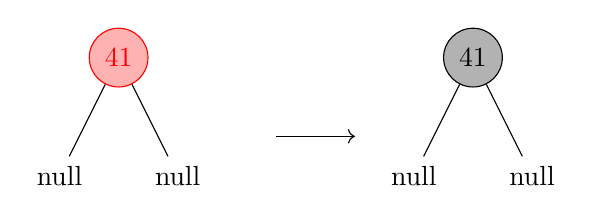
\begin{tikzpicture}
        % Primeiro arvore
        \node[circle, draw=red, fill=red!30, text=red] {41}
            child {node {null}}
            child {node {null}};

        \draw[->] (2,-1) -- (3,-1);

        % Segundo arvore
        \node[circle, draw=black, fill=black!30, shift={(4.5,0)}] {41}
            child {node {null}}
            child {node {null}};
    \end{tikzpicture}
  \end{center}

  \item Inserindo 38:
  \begin{center}
    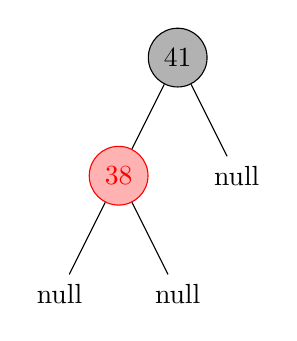
\begin{tikzpicture}
        \node[circle, draw=black, fill=black!30] {41}
            child {
              node[circle, draw=red, fill=red!30, text=red] {38}
                child {node {null}}
                child {node {null}}
            }
            child {node {null}};
    \end{tikzpicture}
  \end{center}
    
  \item Inserindo 31:
  \begin{center}
    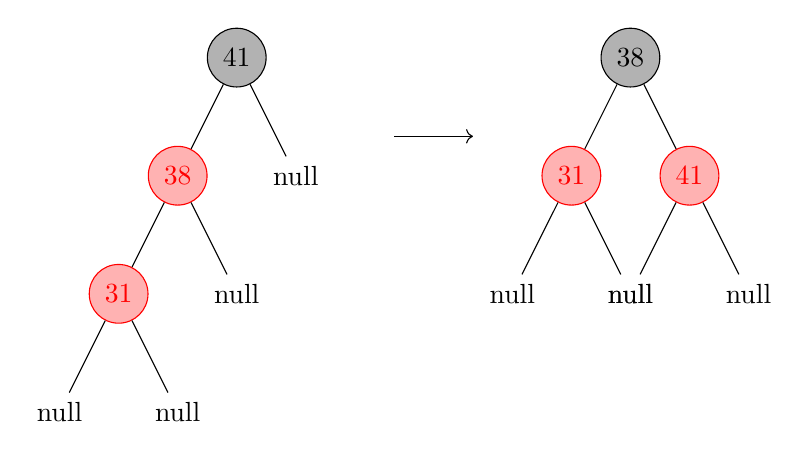
\begin{tikzpicture}
        \node[circle, draw=black, fill=black!30] {41}
            child {
              node[circle, draw=red, fill=red!30, text=red] {38}
                child {
                  node[circle, draw=red, fill=red!30, text=red] {31}
                    child {node {null}}
                    child {node {null}}
                }
                child {node {null}}
            }
            child {node {null}};
        
        \draw[->] (2,-1) -- (3,-1);

        \node[circle, draw=black, fill=black!30, shift={(5,0)}] {38}
            child {
              node[circle, draw=red, fill=red!30, text=red] {31}
                child {node {null}}
                child {node {null}}
            }
            child {
              node[circle, draw=red, fill=red!30, text=red] {41}
                child {node {null}}
                child {node {null}}
            };
    \end{tikzpicture}
  \end{center}
    
  \item Inserindo 12:
  \begin{center}
    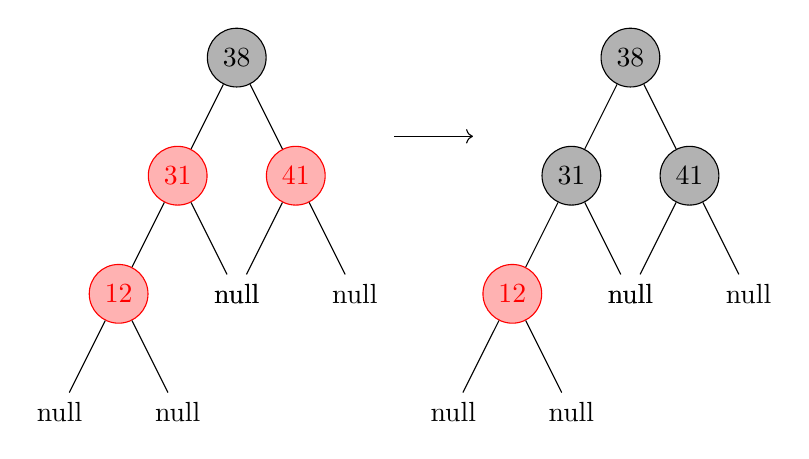
\begin{tikzpicture}
      \node[circle, draw=black, fill=black!30] {38}
        child {
          node[circle, draw=red, fill=red!30, text=red] {31}
            child {
              node[circle, draw=red, fill=red!30, text=red] {12}
                child {node {null}}
                child {node {null}}
            }
            child {node {null}}
        }
        child {
          node[circle, draw=red, fill=red!30, text=red] {41}
            child {node {null}}
            child {node {null}}
        };

      \draw[->] (2,-1) -- (3,-1);

      \node[circle, draw=black, fill=black!30, shift={(5,0)}] {38}
        child {
          node[circle, draw=black, fill=black!30] {31}
            child {
              node[circle, draw=red, fill=red!30, text=red] {12}
                child {node {null}}
                child {node {null}}
            }
            child {node {null}}
        }
        child {
          node[circle, draw=black, fill=black!30] {41}
            child {node {null}}
            child {node {null}}
        };  
    \end{tikzpicture}
  \end{center}
    
  \item Inserindo 19:
  \begin{center}
    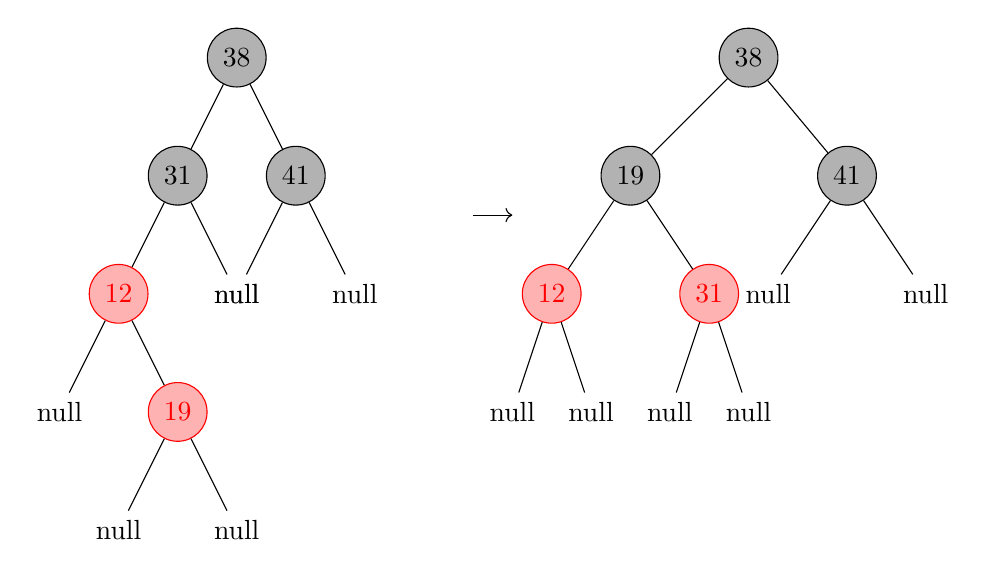
\begin{tikzpicture}
      \node[circle, draw=black, fill=black!30] {38}
        child {
          node[circle, draw=black, fill=black!30] {31}
            child {
              node[circle, draw=red, fill=red!30, text=red] {12}
                child {node {null}}
                child {
                  node[circle, draw=red, fill=red!30, text=red] {19}
                  child {node {null}}
                  child {node {null}}
                }
            }
            child {node {null}}
        }
        child {
          node[circle, draw=black, fill=black!30] {41}
            child {node {null}}
            child {node {null}}
        }; 

      \draw[->] (3,-2) -- (3.5,-2);

      \node[circle, draw=black, fill=black!30, shift={(6.5,0)}] {38}
        child[sibling distance=3cm] {
          node[circle, draw=black, fill=black!30] {19}
            child[sibling distance=2cm] {
              node[circle, draw=red, fill=red!30, text=red] {12}
                child[sibling distance=1cm] {node {null}}
                child[sibling distance=1cm] {node {null}}
            }
            child[sibling distance=2cm] {
              node[circle, draw=red, fill=red!30, text=red] {31}
                child[sibling distance=1cm] {node {null}}
                child[sibling distance=1cm] {node {null}}
            }
        }
        child[sibling distance=2.5cm] {
          node[circle, draw=black, fill=black!30] {41}
            child[sibling distance=2cm] {node {null}}
            child[sibling distance=2cm] {node {null}}
        };  
    \end{tikzpicture}
  \end{center}
    
  \item Inserindo 8:
  \begin{center}
    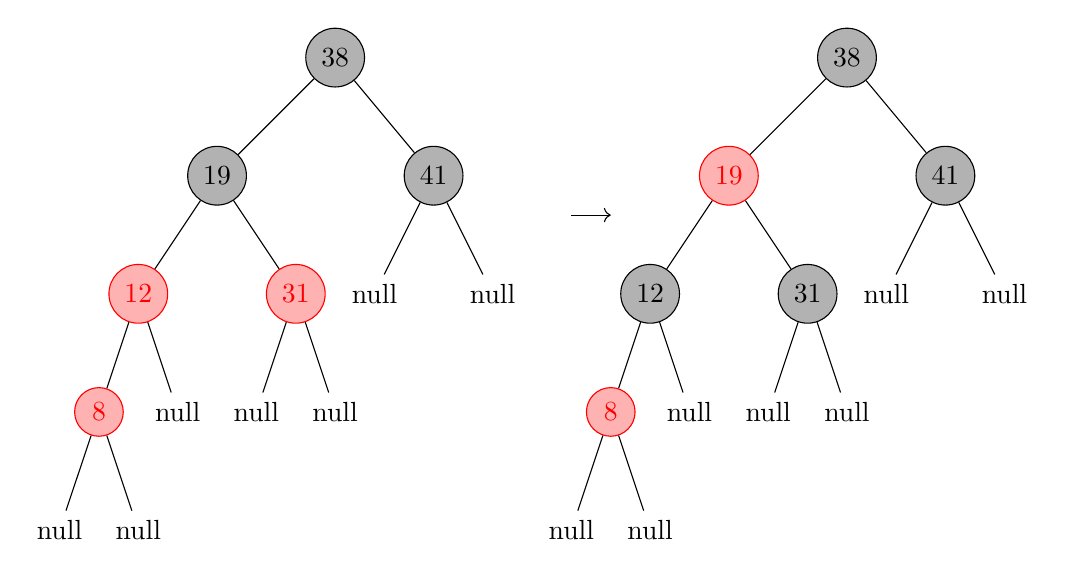
\begin{tikzpicture}
      \node[circle, draw=black, fill=black!30] {38}
        child[sibling distance=3cm] {
          node[circle, draw=black, fill=black!30] {19}
            child[sibling distance=2cm] {
              node[circle, draw=red, fill=red!30, text=red] {12}
                child[sibling distance=1cm] {
                  node[circle, draw=red, fill=red!30, text=red] {8}
                  child[sibling distance=1cm] {node {null}}
                  child[sibling distance=1cm] {node {null}}
                }
                child[sibling distance=1cm] {node {null}}
            }
            child[sibling distance=2cm] {
              node[circle, draw=red, fill=red!30, text=red] {31}
                child[sibling distance=1cm] {node {null}}
                child[sibling distance=1cm] {node {null}}
            }
        }
        child[sibling distance=2.5cm] {
          node[circle, draw=black, fill=black!30] {41}
            child[sibling distance=1.5cm] {node {null}}
            child[sibling distance=1.5cm] {node {null}}
        };  

      \draw[->] (3,-2) -- (3.5,-2);

      \node[circle, draw=black, fill=black!30, shift={(6.5,0)}] {38}
        child[sibling distance=3cm] {
          node[circle, draw=red, fill=red!30, text=red] {19}
            child[sibling distance=2cm] {
              node[circle, draw=black, fill=black!30] {12}
                child[sibling distance=1cm] {
                  node[circle, draw=red, fill=red!30, text=red] {8}
                  child[sibling distance=1cm] {node {null}}
                  child[sibling distance=1cm] {node {null}}
                }
                child[sibling distance=1cm] {node {null}}
            }
            child[sibling distance=2cm] {
              node[circle, draw=black, fill=black!30] {31}
                child[sibling distance=1cm] {node {null}}
                child[sibling distance=1cm] {node {null}}
            }
        }
        child[sibling distance=2.5cm] {
          node[circle, draw=black, fill=black!30] {41}
            child[sibling distance=1.5cm] {node {null}}
            child[sibling distance=1.5cm] {node {null}}
        };  
    \end{tikzpicture}
  \end{center}
    
  \item Inserindo 50:
  \begin{center}
    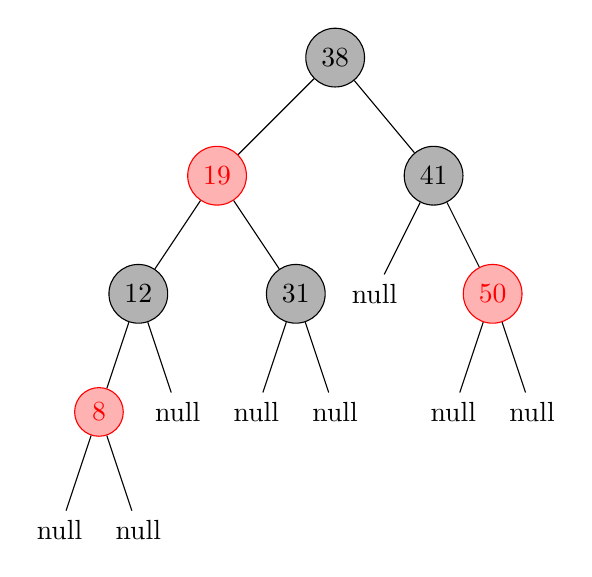
\begin{tikzpicture}
      \node[circle, draw=black, fill=black!30, shift={(6.5,0)}] {38}
        child[sibling distance=3cm] {
          node[circle, draw=red, fill=red!30, text=red] {19}
            child[sibling distance=2cm] {
              node[circle, draw=black, fill=black!30] {12}
                child[sibling distance=1cm] {
                  node[circle, draw=red, fill=red!30, text=red] {8}
                  child[sibling distance=1cm] {node {null}}
                  child[sibling distance=1cm] {node {null}}
                }
                child[sibling distance=1cm] {node {null}}
            }
            child[sibling distance=2cm] {
              node[circle, draw=black, fill=black!30] {31}
                child[sibling distance=1cm] {node {null}}
                child[sibling distance=1cm] {node {null}}
            }
        }
        child[sibling distance=2.5cm] {
          node[circle, draw=black, fill=black!30] {41}
            child[sibling distance=1.5cm] {node {null}}
            child[sibling distance=1.5cm] {
              node[circle, draw=red, fill=red!30, text=red] {50}
              child[sibling distance=1cm] {node {null}}
              child[sibling distance=1cm] {node {null}}
            }
        };
    \end{tikzpicture}
  \end{center}

  \item Inserindo 1:
  \begin{center}
    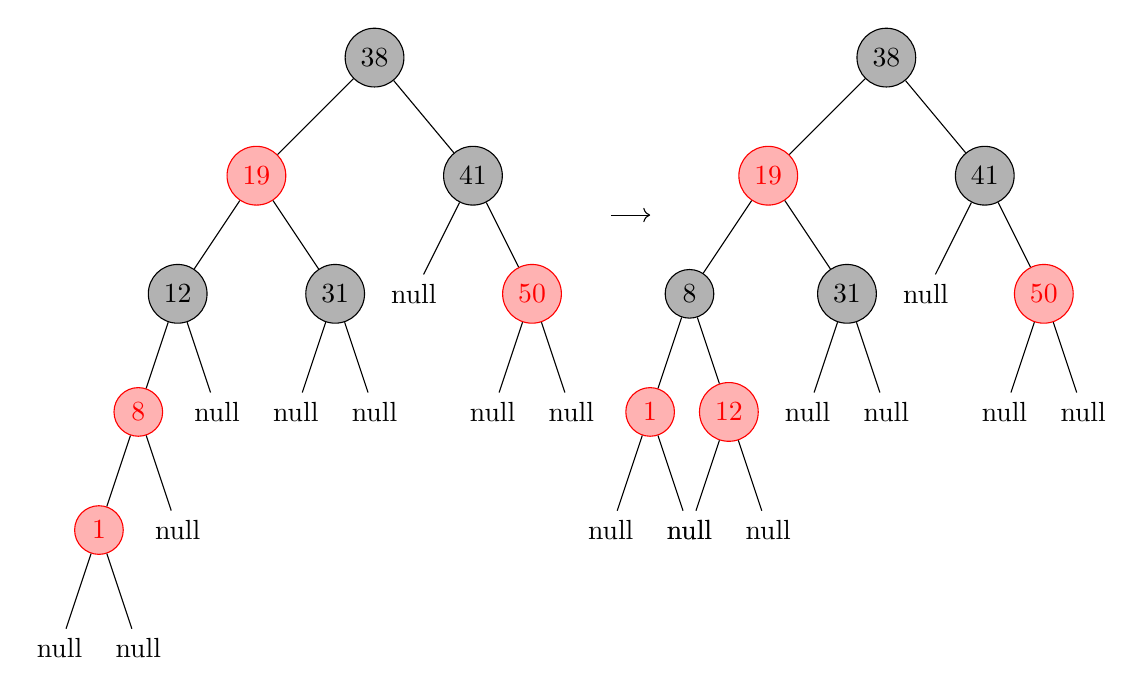
\begin{tikzpicture}
      \node[circle, draw=black, fill=black!30] {38}
        child[sibling distance=3cm] {
          node[circle, draw=red, fill=red!30, text=red] {19}
            child[sibling distance=2cm] {
              node[circle, draw=black, fill=black!30] {12}
                child[sibling distance=1cm] {
                  node[circle, draw=red, fill=red!30, text=red] {8}
                  child[sibling distance=1cm] {
                    node[circle, draw=red, fill=red!30, text=red] {1}
                    child[sibling distance=1cm] {node {null}}
                    child[sibling distance=1cm] {node {null}}
                  }
                  child[sibling distance=1cm] {node {null}}
                }
                child[sibling distance=1cm] {node {null}}
            }
            child[sibling distance=2cm] {
              node[circle, draw=black, fill=black!30] {31}
                child[sibling distance=1cm] {node {null}}
                child[sibling distance=1cm] {node {null}}
            }
        }
        child[sibling distance=2.5cm] {
          node[circle, draw=black, fill=black!30] {41}
            child[sibling distance=1.5cm] {node {null}}
            child[sibling distance=1.5cm] {
              node[circle, draw=red, fill=red!30, text=red] {50}
              child[sibling distance=1cm] {node {null}}
              child[sibling distance=1cm] {node {null}}
            }
        };

      \draw[->] (3,-2) -- (3.5,-2);

      \node[circle, draw=black, fill=black!30, shift={(6.5,0)}] {38}
        child[sibling distance=3cm] {
          node[circle, draw=red, fill=red!30, text=red] {19}
            child[sibling distance=2cm] {
              node[circle, draw=black, fill=black!30] {8}
                child[sibling distance=1cm] {
                  node[circle, draw=red, fill=red!30, text=red] {1}
                    child[sibling distance=1cm] {node {null}}
                    child[sibling distance=1cm] {node {null}}
                }
                child[sibling distance=1cm] {
                  node[circle, draw=red, fill=red!30, text=red] {12}
                  child[sibling distance=1cm] {node {null}}
                  child[sibling distance=1cm] {node {null}}
                }
            }
            child[sibling distance=2cm] {
              node[circle, draw=black, fill=black!30] {31}
                child[sibling distance=1cm] {node {null}}
                child[sibling distance=1cm] {node {null}}
            }
        }
        child[sibling distance=2.5cm] {
          node[circle, draw=black, fill=black!30] {41}
            child[sibling distance=1.5cm] {node {null}}
            child[sibling distance=1.5cm] {
              node[circle, draw=red, fill=red!30, text=red] {50}
              child[sibling distance=1cm] {node {null}}
              child[sibling distance=1cm] {node {null}}
            }
        };
    \end{tikzpicture}
  \end{center}

  \item Inserindo 100:
  \begin{center}
    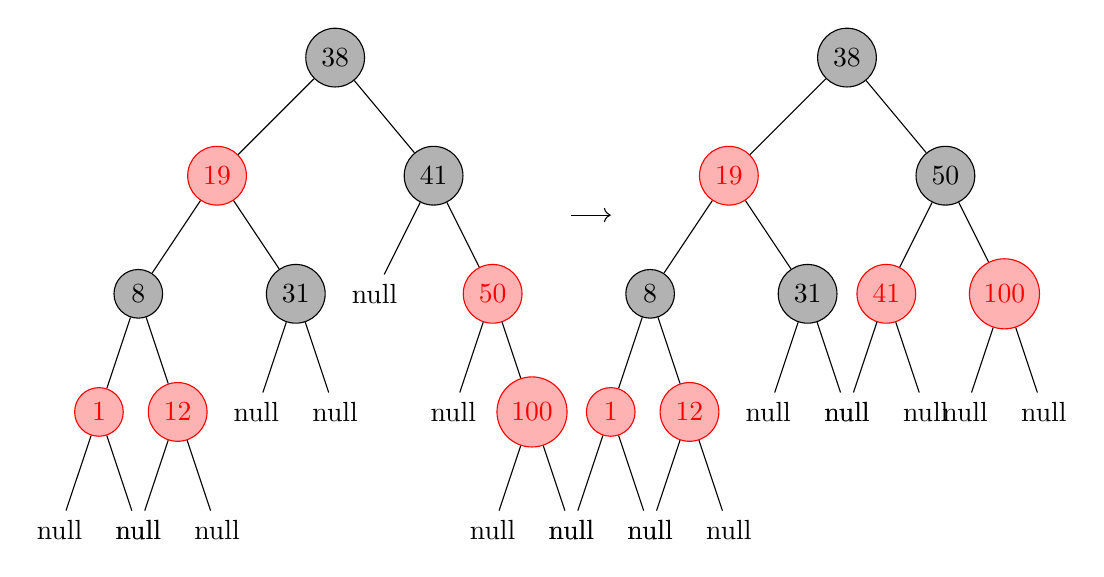
\begin{tikzpicture}
      \node[circle, draw=black, fill=black!30] {38}
        child[sibling distance=3cm] {
          node[circle, draw=red, fill=red!30, text=red] {19}
            child[sibling distance=2cm] {
              node[circle, draw=black, fill=black!30] {8}
                child[sibling distance=1cm] {
                  node[circle, draw=red, fill=red!30, text=red] {1}
                    child[sibling distance=1cm] {node {null}}
                    child[sibling distance=1cm] {node {null}}
                }
                child[sibling distance=1cm] {
                  node[circle, draw=red, fill=red!30, text=red] {12}
                  child[sibling distance=1cm] {node {null}}
                  child[sibling distance=1cm] {node {null}}
                }
            }
            child[sibling distance=2cm] {
              node[circle, draw=black, fill=black!30] {31}
                child[sibling distance=1cm] {node {null}}
                child[sibling distance=1cm] {node {null}}
            }
        }
        child[sibling distance=2.5cm] {
          node[circle, draw=black, fill=black!30] {41}
            child[sibling distance=1.5cm] {node {null}}
            child[sibling distance=1.5cm] {
              node[circle, draw=red, fill=red!30, text=red] {50}
              child[sibling distance=1cm] {node {null}}
              child[sibling distance=1cm] {
                node[circle, draw=red, fill=red!30, text=red] {100}
                child[sibling distance=1cm] {node {null}}
                child[sibling distance=1cm] {node {null}}
              }
            }
        };

      \draw[->] (3,-2) -- (3.5,-2);

      \node[circle, draw=black, fill=black!30, shift={(6.5,0)}] {38}
        child[sibling distance=3cm] {
          node[circle, draw=red, fill=red!30, text=red] {19}
            child[sibling distance=2cm] {
              node[circle, draw=black, fill=black!30] {8}
                child[sibling distance=1cm] {
                  node[circle, draw=red, fill=red!30, text=red] {1}
                    child[sibling distance=1cm] {node {null}}
                    child[sibling distance=1cm] {node {null}}
                }
                child[sibling distance=1cm] {
                  node[circle, draw=red, fill=red!30, text=red] {12}
                  child[sibling distance=1cm] {node {null}}
                  child[sibling distance=1cm] {node {null}}
                }
            }
            child[sibling distance=2cm] {
              node[circle, draw=black, fill=black!30] {31}
                child[sibling distance=1cm] {node {null}}
                child[sibling distance=1cm] {node {null}}
            }
        }
        child[sibling distance=2.5cm] {
          node[circle, draw=black, fill=black!30] {50}
            child[sibling distance=1.5cm] {
              node[circle, draw=red, fill=red!30, text=red] {41}
              child[sibling distance=1cm] {node {null}}
              child[sibling distance=1cm] {node {null}}
            }
            child[sibling distance=1.5cm] {
              node[circle, draw=red, fill=red!30, text=red] {100}
              child[sibling distance=1cm] {node {null}}
              child[sibling distance=1cm] {node {null}}
            }
        };
    \end{tikzpicture}
  \end{center}

  \item Inserindo 101:
  \begin{center}
    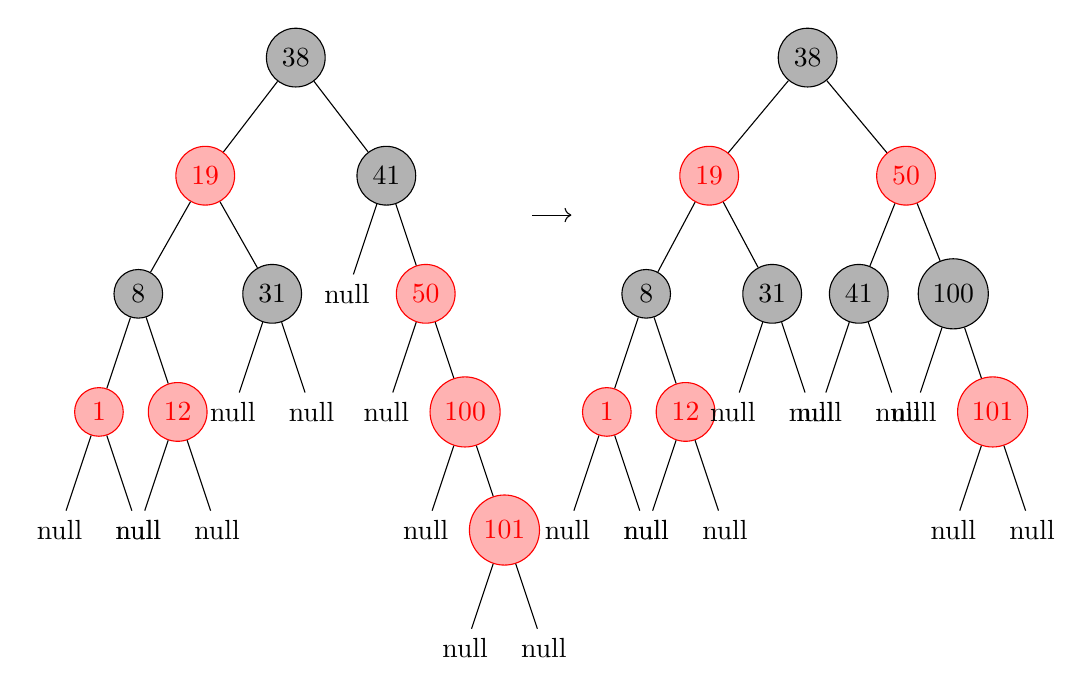
\begin{tikzpicture}
      \node[circle, draw=black, fill=black!30] {38}
        child[sibling distance=2.3cm] {
          node[circle, draw=red, fill=red!30, text=red] {19}
            child[sibling distance=1.7cm] {
              node[circle, draw=black, fill=black!30] {8}
                child[sibling distance=1cm] {
                  node[circle, draw=red, fill=red!30, text=red] {1}
                    child[sibling distance=1cm] {node {null}}
                    child[sibling distance=1cm] {node {null}}
                }
                child[sibling distance=1cm] {
                  node[circle, draw=red, fill=red!30, text=red] {12}
                  child[sibling distance=1cm] {node {null}}
                  child[sibling distance=1cm] {node {null}}
                }
            }
            child[sibling distance=1.7cm] {
              node[circle, draw=black, fill=black!30] {31}
                child[sibling distance=1cm] {node {null}}
                child[sibling distance=1cm] {node {null}}
            }
        }
        child[sibling distance=2.3cm] {
          node[circle, draw=black, fill=black!30] {41}
            child[sibling distance=1cm] {node {null}}
            child[sibling distance=1cm] {
              node[circle, draw=red, fill=red!30, text=red] {50}
              child[sibling distance=1cm] {node {null}}
              child[sibling distance=1cm] {
                node[circle, draw=red, fill=red!30, text=red] {100}
                child[sibling distance=1cm] {node {null}}
                child[sibling distance=1cm] {
                  node[circle, draw=red, fill=red!30, text=red] {101}
                  child[sibling distance=1cm] {node {null}}
                  child[sibling distance=1cm] {node {null}}
                }
              }
            }
        };

      \draw[->] (3,-2) -- (3.5,-2);

      \node[circle, draw=black, fill=black!30, shift={(6.5,0)}] {38}
        child[sibling distance=2.5cm] {
          node[circle, draw=red, fill=red!30, text=red] {19}
            child[sibling distance=1.6cm] {
              node[circle, draw=black, fill=black!30] {8}
                child[sibling distance=1cm] {
                  node[circle, draw=red, fill=red!30, text=red] {1}
                    child[sibling distance=1cm] {node {null}}
                    child[sibling distance=1cm] {node {null}}
                }
                child[sibling distance=1cm] {
                  node[circle, draw=red, fill=red!30, text=red] {12}
                  child[sibling distance=1cm] {node {null}}
                  child[sibling distance=1cm] {node {null}}
                }
            }
            child[sibling distance=1.6cm] {
              node[circle, draw=black, fill=black!30] {31}
                child[sibling distance=1cm] {node {null}}
                child[sibling distance=1cm] {node {null}}
            }
        }
        child[sibling distance=2.5cm] {
          node[circle, draw=red, fill=red!30, text=red] {50}
            child[sibling distance=1.2cm] {
              node[circle, draw=black, fill=black!30] {41}
              child[sibling distance=1cm] {node {null}}
              child[sibling distance=1cm] {node {null}}
            }
            child[sibling distance=1.2cm] {
              node[circle, draw=black, fill=black!30] {100}
              child[sibling distance=1cm] {node {null}}
              child[sibling distance=1cm] {
                node[circle, draw=red, fill=red!30, text=red] {101}
                child[sibling distance=1cm] {node {null}}
                child[sibling distance=1cm] {node {null}}
              }
            }
        };
    \end{tikzpicture}
  \end{center}

\end{enumerate}

\subsubsection{(0,4) Desenhe o passo-a-passo com remoção dos elementos 50 e 8 na árvore
anterior.}

\begin{enumerate}
  \item Removendo 50:
  \begin{center}
    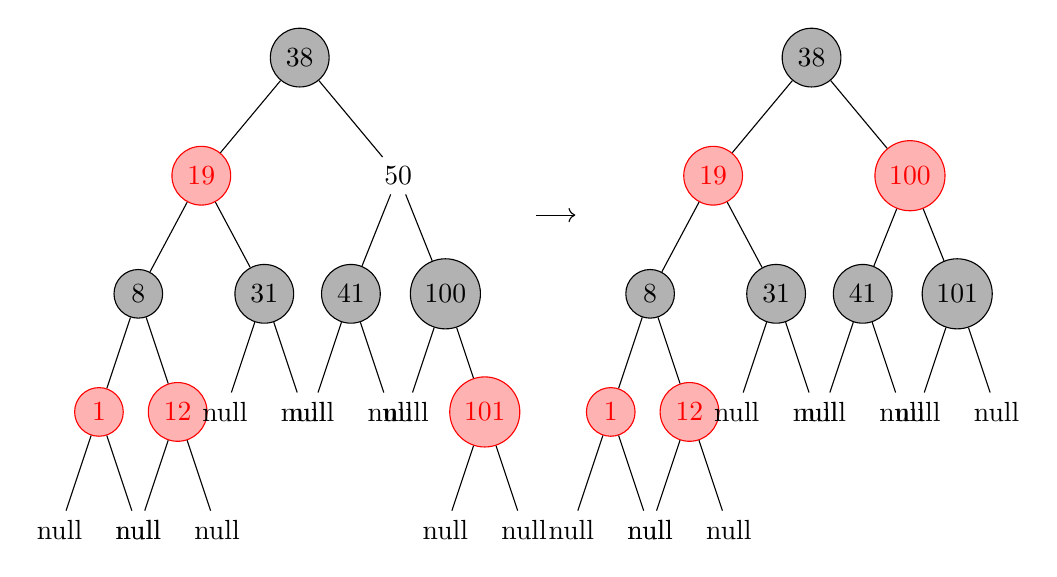
\begin{tikzpicture}
      \node[circle, draw=black, fill=black!30] {38}
        child[sibling distance=2.5cm] {
          node[circle, draw=red, fill=red!30, text=red] {19}
            child[sibling distance=1.6cm] {
              node[circle, draw=black, fill=black!30] {8}
                child[sibling distance=1cm] {
                  node[circle, draw=red, fill=red!30, text=red] {1}
                    child[sibling distance=1cm] {node {null}}
                    child[sibling distance=1cm] {node {null}}
                }
                child[sibling distance=1cm] {
                  node[circle, draw=red, fill=red!30, text=red] {12}
                  child[sibling distance=1cm] {node {null}}
                  child[sibling distance=1cm] {node {null}}
                }
            }
            child[sibling distance=1.6cm] {
              node[circle, draw=black, fill=black!30] {31}
                child[sibling distance=1cm] {node {null}}
                child[sibling distance=1cm] {node {null}}
            }
        }
        child[sibling distance=2.5cm] {
          node{50}
            child[sibling distance=1.2cm] {
              node[circle, draw=black, fill=black!30] {41}
              child[sibling distance=1cm] {node {null}}
              child[sibling distance=1cm] {node {null}}
            }
            child[sibling distance=1.2cm] {
              node[circle, draw=black, fill=black!30] {100}
              child[sibling distance=1cm] {node {null}}
              child[sibling distance=1cm] {
                node[circle, draw=red, fill=red!30, text=red] {101}
                child[sibling distance=1cm] {node {null}}
                child[sibling distance=1cm] {node {null}}
              }
            }
        };

      \draw[->] (3,-2) -- (3.5,-2);

      \node[circle, draw=black, fill=black!30, shift={(6.5,0)}] {38}
        child[sibling distance=2.5cm] {
          node[circle, draw=red, fill=red!30, text=red] {19}
            child[sibling distance=1.6cm] {
              node[circle, draw=black, fill=black!30] {8}
                child[sibling distance=1cm] {
                  node[circle, draw=red, fill=red!30, text=red] {1}
                    child[sibling distance=1cm] {node {null}}
                    child[sibling distance=1cm] {node {null}}
                }
                child[sibling distance=1cm] {
                  node[circle, draw=red, fill=red!30, text=red] {12}
                  child[sibling distance=1cm] {node {null}}
                  child[sibling distance=1cm] {node {null}}
                }
            }
            child[sibling distance=1.6cm] {
              node[circle, draw=black, fill=black!30] {31}
                child[sibling distance=1cm] {node {null}}
                child[sibling distance=1cm] {node {null}}
            }
        }
        child[sibling distance=2.5cm] {
          node[circle, draw=red, fill=red!30, text=red] {100}
            child[sibling distance=1.2cm] {
              node[circle, draw=black, fill=black!30] {41}
              child[sibling distance=1cm] {node {null}}
              child[sibling distance=1cm] {node {null}}
            }
            child[sibling distance=1.2cm] {
              node[circle, draw=black, fill=black!30] {101}
              child[sibling distance=1cm] {node {null}}
              child[sibling distance=1cm] {node {null}}
            }
        };
    \end{tikzpicture}
  \end{center}
    
  \item Removendo 8:
  \begin{center}
    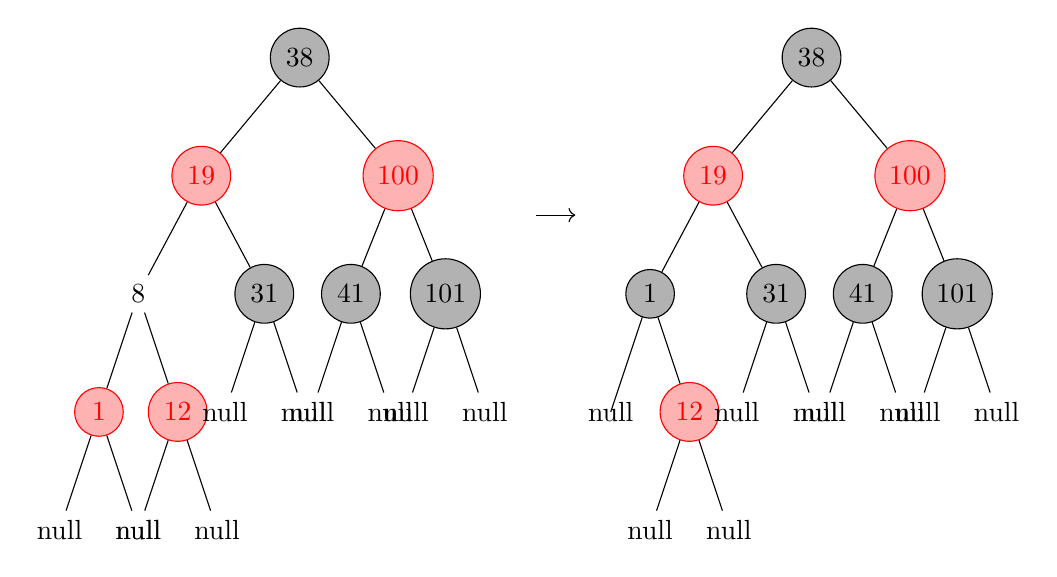
\begin{tikzpicture}
      \node[circle, draw=black, fill=black!30] {38}
        child[sibling distance=2.5cm] {
          node[circle, draw=red, fill=red!30, text=red] {19}
            child[sibling distance=1.6cm] {
              node {8}
                child[sibling distance=1cm] {
                  node[circle, draw=red, fill=red!30, text=red] {1}
                    child[sibling distance=1cm] {node {null}}
                    child[sibling distance=1cm] {node {null}}
                }
                child[sibling distance=1cm] {
                  node[circle, draw=red, fill=red!30, text=red] {12}
                  child[sibling distance=1cm] {node {null}}
                  child[sibling distance=1cm] {node {null}}
                }
            }
            child[sibling distance=1.6cm] {
              node[circle, draw=black, fill=black!30] {31}
                child[sibling distance=1cm] {node {null}}
                child[sibling distance=1cm] {node {null}}
            }
        }
        child[sibling distance=2.5cm] {
          node[circle, draw=red, fill=red!30, text=red] {100}
            child[sibling distance=1.2cm] {
              node[circle, draw=black, fill=black!30] {41}
              child[sibling distance=1cm] {node {null}}
              child[sibling distance=1cm] {node {null}}
            }
            child[sibling distance=1.2cm] {
              node[circle, draw=black, fill=black!30] {101}
              child[sibling distance=1cm] {node {null}}
              child[sibling distance=1cm] {node {null}}
            }
        };

      \draw[->] (3,-2) -- (3.5,-2);

      \node[circle, draw=black, fill=black!30, shift={(6.5,0)}] {38}
        child[sibling distance=2.5cm] {
          node[circle, draw=red, fill=red!30, text=red] {19}
            child[sibling distance=1.6cm] {
              node[circle, draw=black, fill=black!30] {1}
                child[sibling distance=1cm] {{node {null}}}
                child[sibling distance=1cm] {
                  node[circle, draw=red, fill=red!30, text=red] {12}
                  child[sibling distance=1cm] {node {null}}
                  child[sibling distance=1cm] {node {null}}
                }
            }
            child[sibling distance=1.6cm] {
              node[circle, draw=black, fill=black!30] {31}
                child[sibling distance=1cm] {node {null}}
                child[sibling distance=1cm] {node {null}}
            }
        }
        child[sibling distance=2.5cm] {
          node[circle, draw=red, fill=red!30, text=red] {100}
            child[sibling distance=1.2cm] {
              node[circle, draw=black, fill=black!30] {41}
              child[sibling distance=1cm] {node {null}}
              child[sibling distance=1cm] {node {null}}
            }
            child[sibling distance=1.2cm] {
              node[circle, draw=black, fill=black!30] {101}
              child[sibling distance=1cm] {node {null}}
              child[sibling distance=1cm] {node {null}}
            }
        };
    \end{tikzpicture}
  \end{center}

\end{enumerate}

\subsubsection{(0,2) Explique as principais diferenças entre árvores AVL e vermelho-preto.}

\subsubsection{Solução:}

Fonte: ChatGPT
\\
\\Principais Diferenças:
  \begin{enumerate}[label=\alph*)]
    \item Balanceamento: 
    \begin{itemize}
      \item As árvores AVL são árvores binárias de busca auto-balanceadas que mantêm um critério de balanceamento mais rigoroso, garantindo que a diferença de altura (fator de balanceamento) entre as subárvores esquerda e direita de qualquer nó não seja maior que 1.
      \item Em contraste, as árvores vermelho-preto são menos rigorosas no balanceamento, pois permitem que as subárvores de um nó diferenciem em altura em até um fator logarítmico (log n), o que resulta em uma árvore mais relaxada em relação ao balanceamento.
    \end{itemize}
    \item Rotações:
      \begin{itemize}
        \item As árvores AVL requerem mais rotações para manter o balanceamento devido ao seu critério mais restritivo. Portanto, operações de inserção e remoção podem demandar mais tempo de reestruturação.
        \item Em árvores vermelho-preto, o balanceamento menos rígido reduz a necessidade de rotações. Geralmente, essas árvores realizam menos rotações durante as operações, tornando-as mais rápidas em cenários onde são necessárias muitas inserções e deleções.
      \end{itemize}
    \item Eficiência de Busca e Atualização::
      \begin{itemize}
        \item As árvores AVL, devido ao seu balanceamento mais rígido, tendem a ser mais eficientes em operações de busca, pois a altura da árvore é mantida menor que nas árvores vermelho-preto.
        \item As árvores vermelho-preto, por outro lado, podem ser mais eficientes para cenários que exigem inserções e deleções frequentes, já que o balanceamento mais flexível reduz o número de rotações e ajustes.
      \end{itemize}
    \item Aplicações:
      \begin{itemize}
        \item Devido à eficiência em busca, as árvores AVL são preferidas em aplicativos onde as operações de leitura (busca) são mais comuns que as operações de escrita (inserção e remoção).
        \item As árvores vermelho-preto são amplamente usadas em estruturas como tabelas de símbolos e ambientes de compiladores, onde tanto a leitura quanto a escrita ocorrem frequentemente.
      \end{itemize}
  \end{enumerate}
\end{document}